\documentclass[tikz,border=10pt]{standalone}
\usepackage{amsmath}
\begin{document}
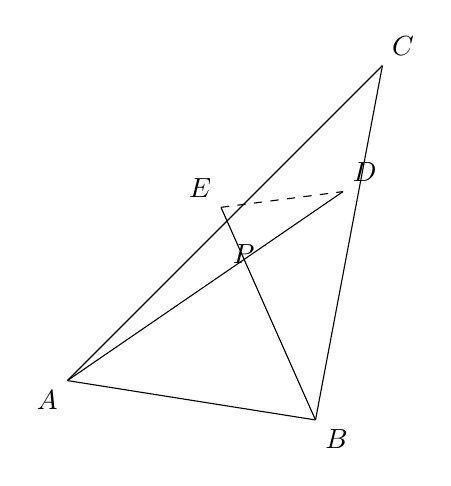
\begin{tikzpicture}[scale=0.05]
\coordinate (A) at (0,0);
\coordinate (B) at (63,-10);
\coordinate (C) at (80,80);
\coordinate (E) at (39,44);
\coordinate (D) at (70,48);
\coordinate (P) at (50,37);

\draw (A) -- (B);
\draw (B) -- (C);
\draw (C) -- (A);
\draw (E) -- (B);
\draw (A) -- (D);
\draw[dashed] (E) -- (D);

\node[above left] at (E) {$E$};
\node[above right] at (D) {$D$};
\node[below left] at (P) {$P$};
\node[below left] at (A) {$A$};
\node[below right] at (B) {$B$};
\node[above right] at (C) {$C$};
\end{tikzpicture}
\end{document}
